\chapter{Existing solutions}
\label{chapter:solutions}
The urban data visualization process can be viewed from multiple perspectives. We can consider the actual physical form of the presentation --- the medium and the the interaction mechanism. On the other hand, it is possible to consider the tools used for the visualization creation, which is more closely related to the standard visualization pipeline. Considering the physical form of the visualization, the examples listed in this chapter can be divided into categories --- purely virtual visualizations, and visualizations with physical components.

\section{Visualization Tools with Physical Components}
This section presents a selected list of visualization tools and projects which use interactive physical components in any shape or form. Due to the nature of these tools, the environment where the visualization is presented plays an important role. It has a profound influence on accessibility, interactivity, and the overall user experience. All presented examples share a common scheme --- a table with interactive physical components is accompanied by a wide-screen projection presenting the actual visualization.   

\paragraph{Tactile Matrix}
Ira Winder and Kent Larson have presented a framework called Tactile Matrix \cite{winderTangible2017}. It is a collaborative tool for real-time computation and projection mapping, see figure \ref{fig:tactilematrix}. The tool is based on a principle described in section \ref{sec:analytics}. The users are presented with a matrix representing city blocks; additional information is conveyed by the visualization projected on top of the matrix. The visualization is driven by an analytical model, which takes the matrix configuration as an input. Lego blocks can be placed into the matrix and the system updates the projection, as the model responds to new inputs. The tool is implemented in Processing, which is a Java-based environment. The SDK for the Tactile Matrix project is available, which also includes the manual to construct the physical components.

\begin{figure}[h]
    \centering
    \begin{subfigure}[t]{0.49\linewidth}
        \centering
        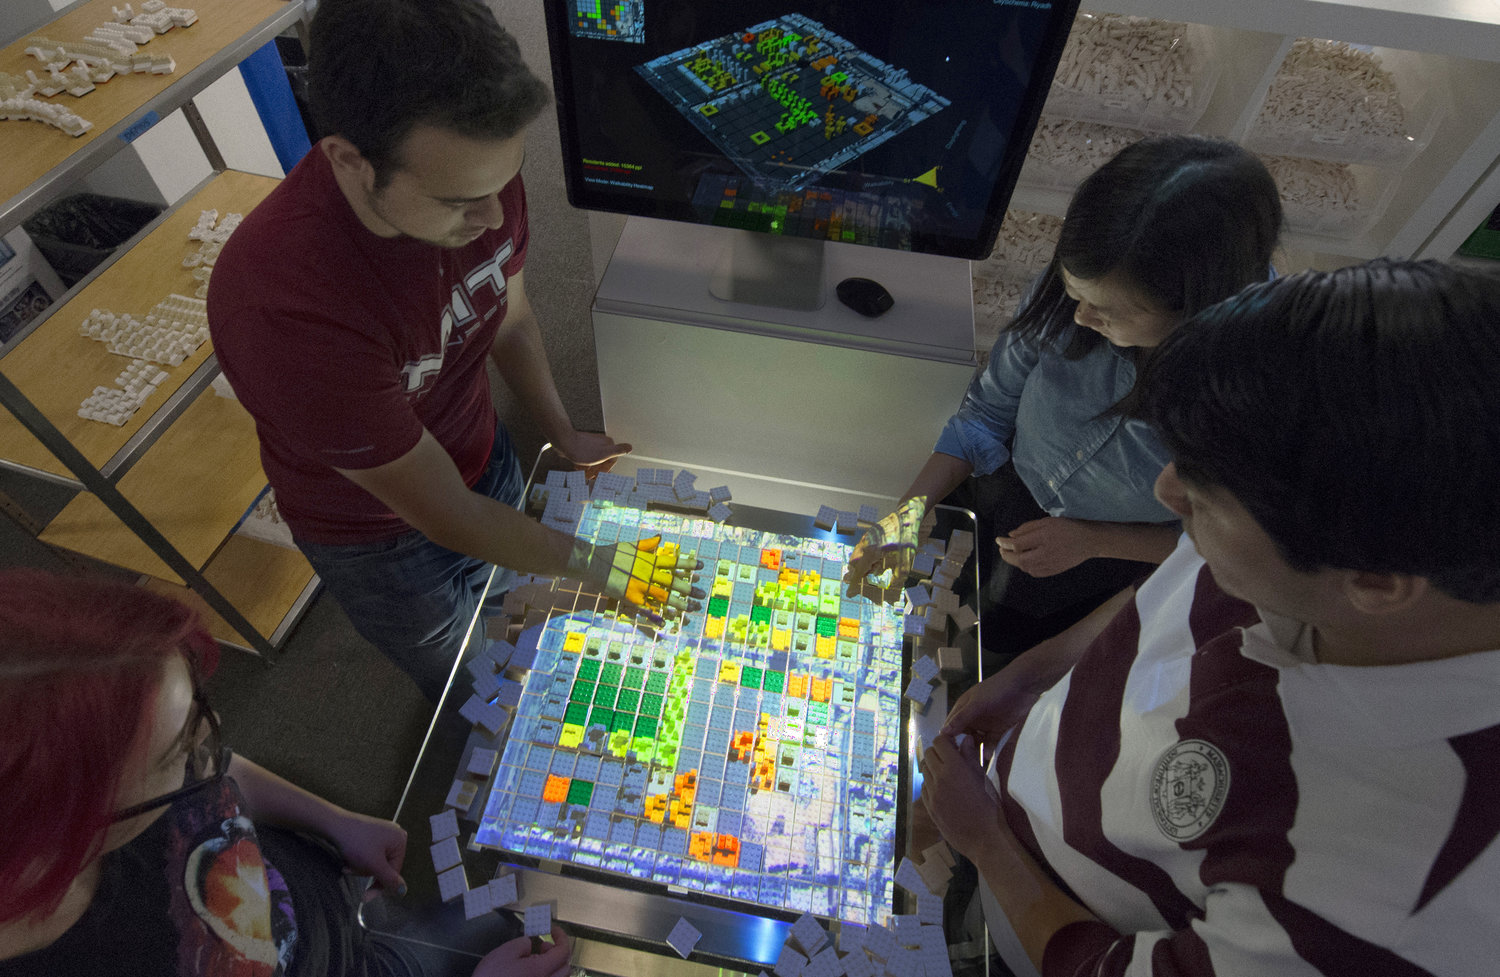
\includegraphics[width=\linewidth]{figures/tactile.jpg}
        \caption{Participants using Tactile Matrix \cite{winderTactileUsers}}
    \end{subfigure}
    \begin{subfigure}[t]{0.49\linewidth}
        \centering
        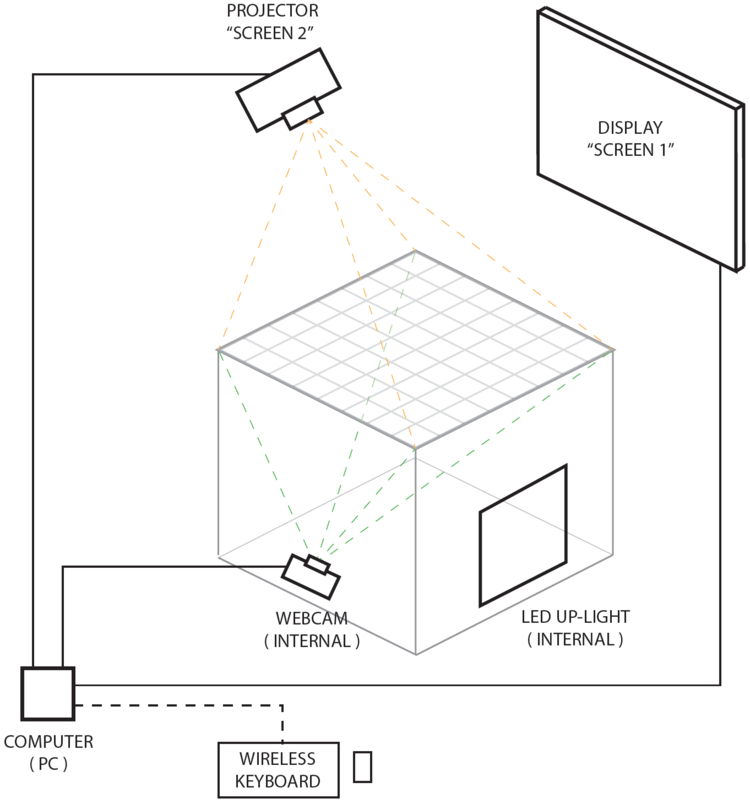
\includegraphics[width=0.6\linewidth]{figures/tactilematrixelectronics.png}
        \caption{SDK Scheme \cite{winderTactileScheme}}
    \end{subfigure}
    \caption{Tactile Matrix framework}
    \label{fig:tactilematrix}
\end{figure}

\paragraph{Pře(d)stav si Prahu} 
In 2019, the OFICINA studio created for IPR Prague an interactive exhibition \cite{oficinaPredstav}. The exhibition aimed to present Strategic Plan for Prague \cite{pragueStrategicPlan}. The visitors had the opportunity to try the role of city planners. The exhibition used the space of the Center for Architecture and Metropolitan Planning (CAMP). The dominant feature of the exhibition was the wide-screen projection displaying the current state of the simulation, see figure \ref{fig:oficinaexhib}. The task of the visitors was to regulate the city life (e.g. tourism, transport), and set the course of the future development (e.g. investments, housing). The simulation was controlled by the amount of colorful blocks on tables (see figure \ref{fig:oficinablocks}), and by analog pulls. Each analog control was assigned a specific action; placing the block or activating the pull sent a new input to the underlying model. The wide-screen visualization provided the visual feedback. The virtual visual components were implemented using web technologies to provide more flexibility.

\begin{figure}[h]
    \centering
    \begin{subfigure}[t]{0.49\linewidth}
        \centering
        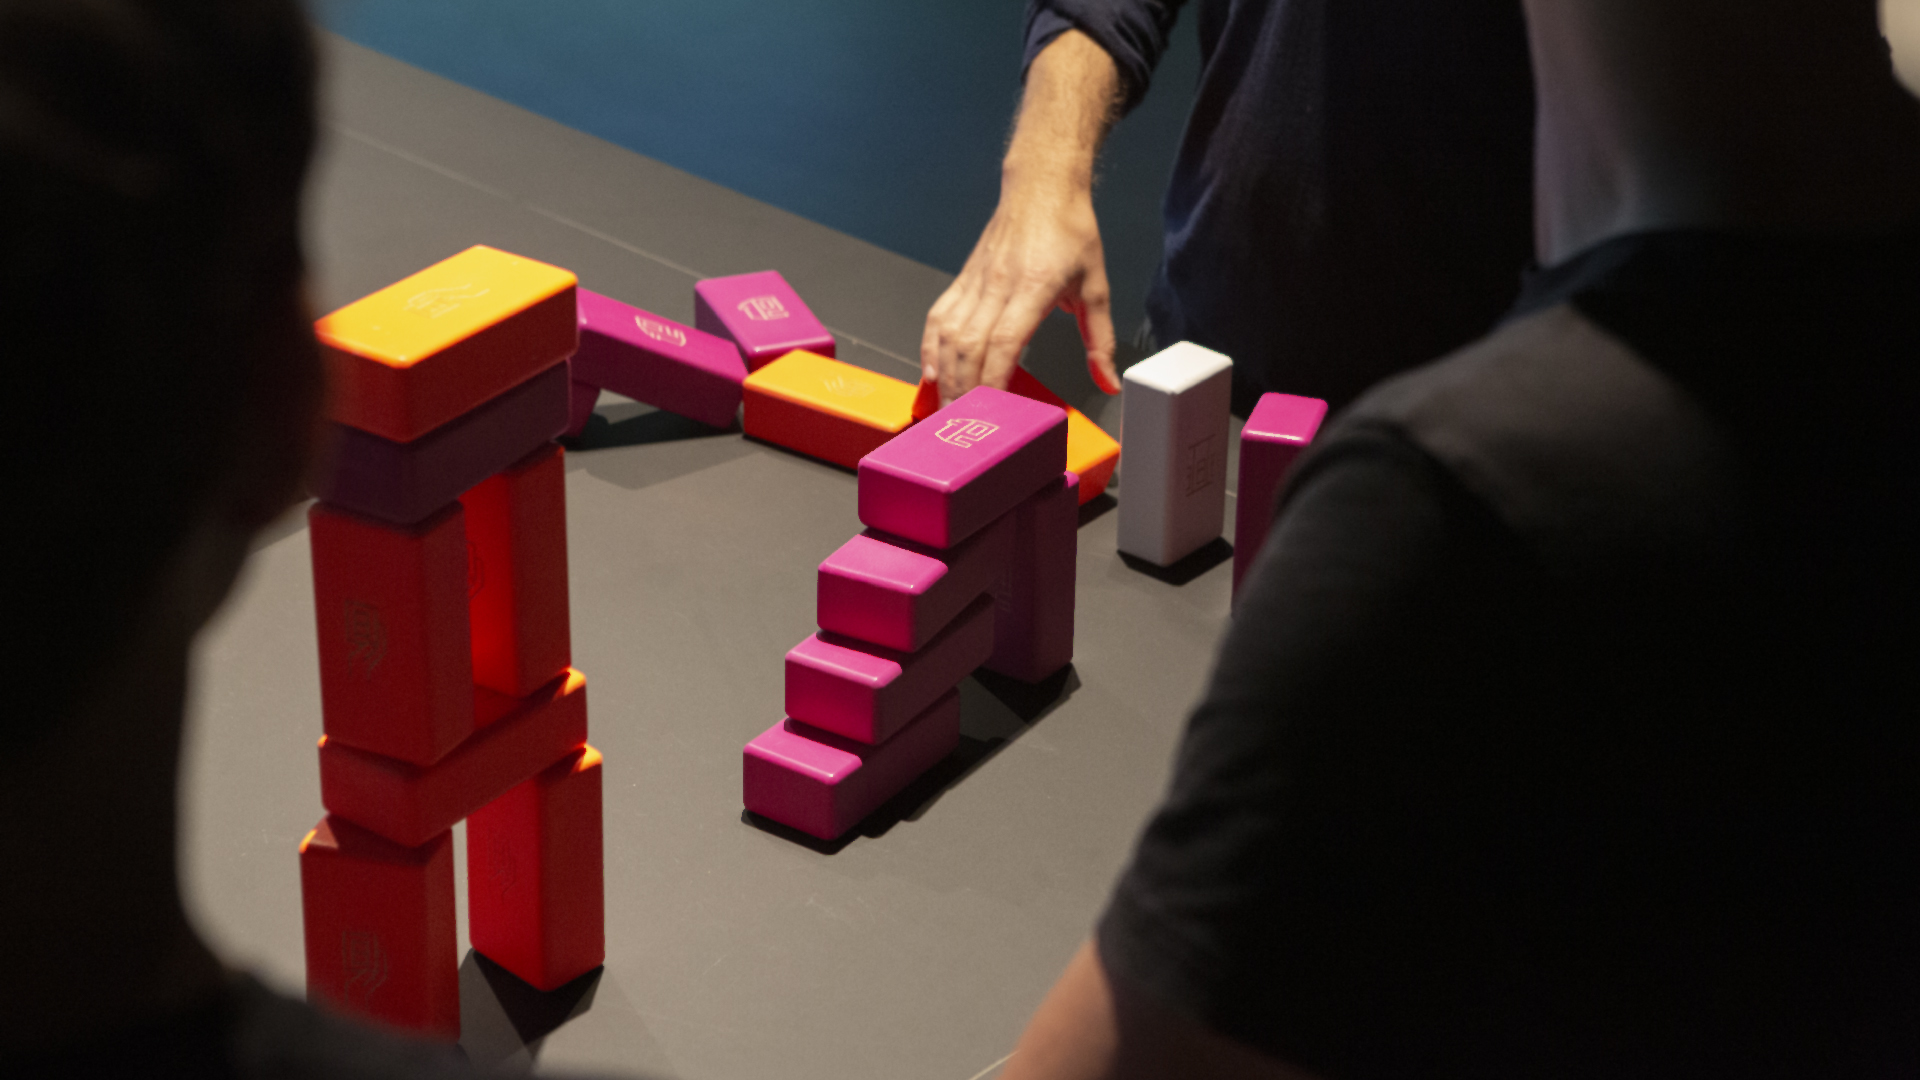
\includegraphics[width=\linewidth]{figures/oficina1.jpg}
        \caption{Color blocks \cite{oficinaPredstav}}
        \label{fig:oficinablocks}
    \end{subfigure}
    \begin{subfigure}[t]{0.49\linewidth}
        \centering
        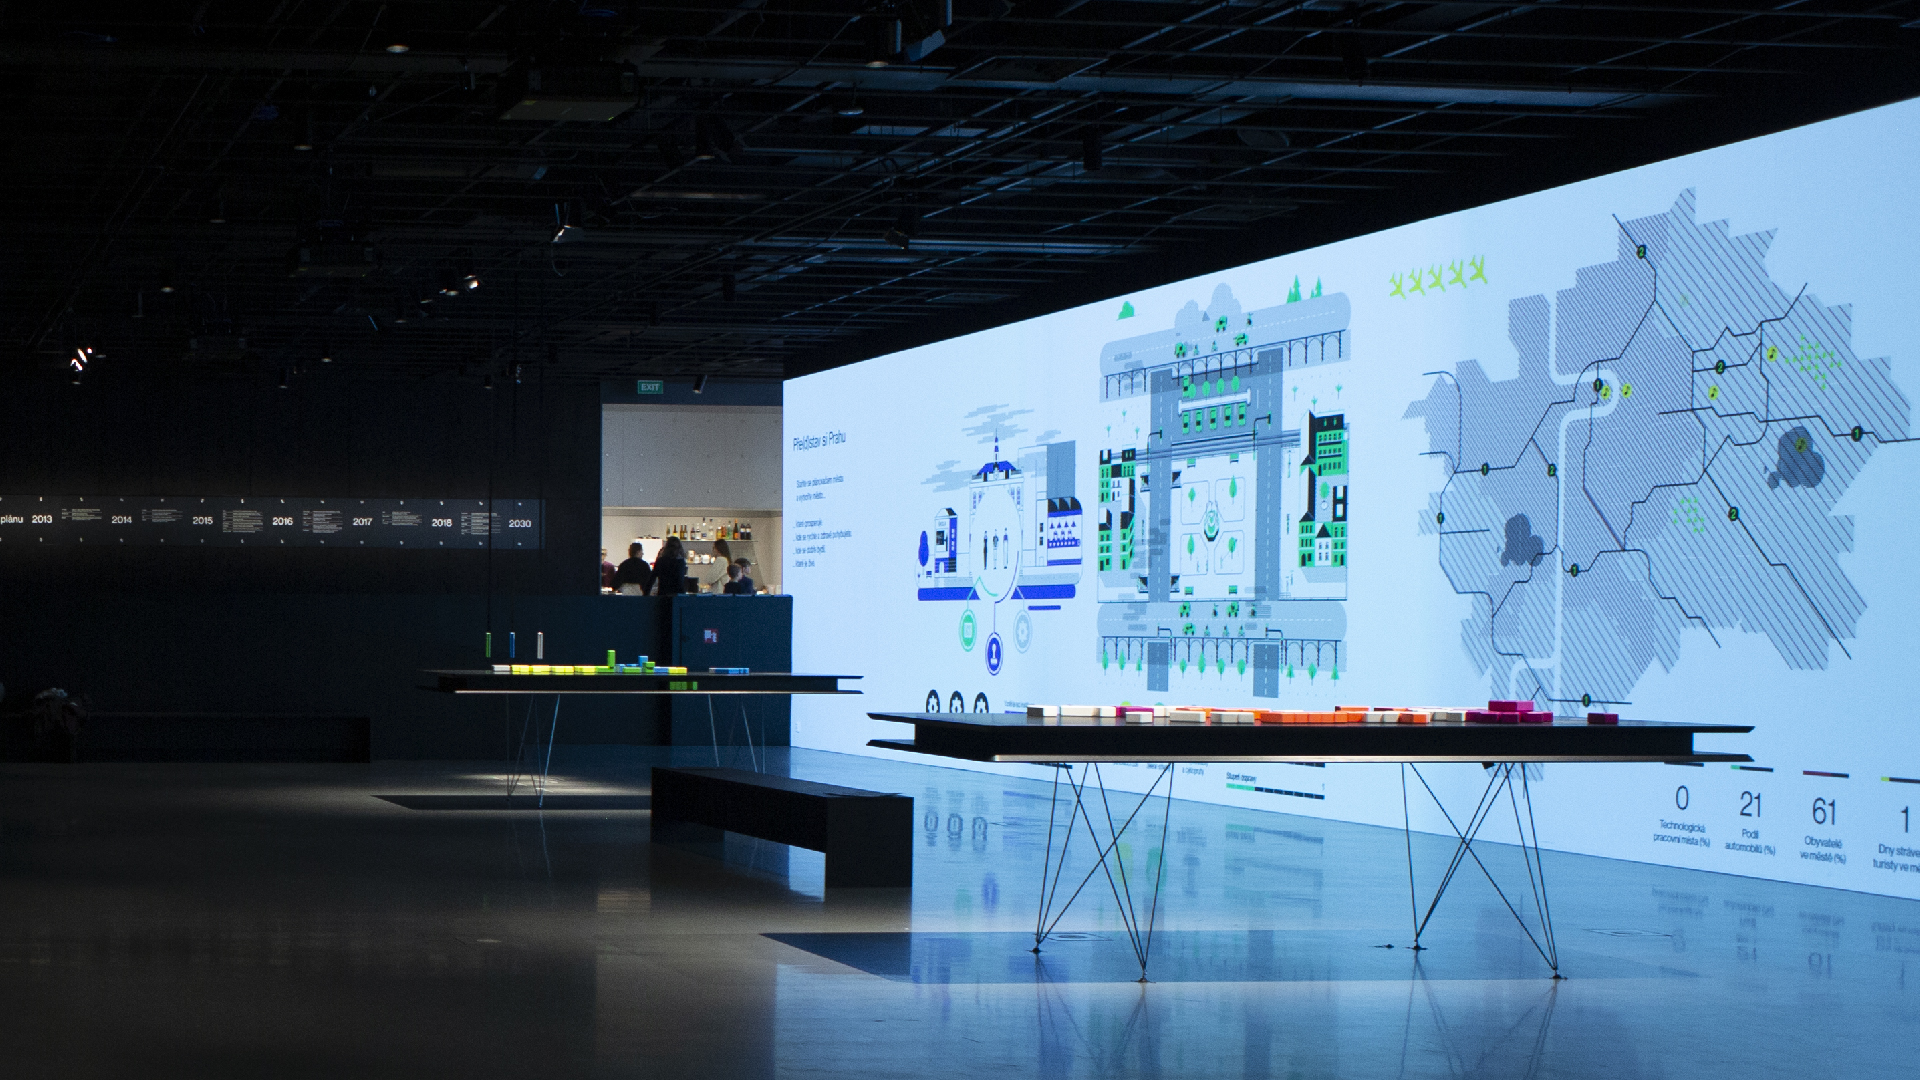
\includegraphics[width=\linewidth]{figures/oficina2.jpg}
        \caption{The exhibition environment \cite{oficinaPredstav}}
        \label{fig:oficinaexhib}
    \end{subfigure}
    \caption{Pře(d)stav si Prahu by OFICINA in CAMP}
    \label{fig:oficinapredstav}
\end{figure}


\paragraph{Rohanský ostrov: nový Karlín?} 
Another exhibition at CAMP in 2019 used a combination of architectural model and projection mapping, more details can be found in \cite{iprRohan}. The exhibition was not interactive; however, the projection served as a visual aid for the visitors standing around the physical model. The projection highlited areas and buildings that will be transformed in the next 20 years.

\begin{figure}[h]
    \centering
    \begin{subfigure}[t]{0.49\linewidth}
        \centering
        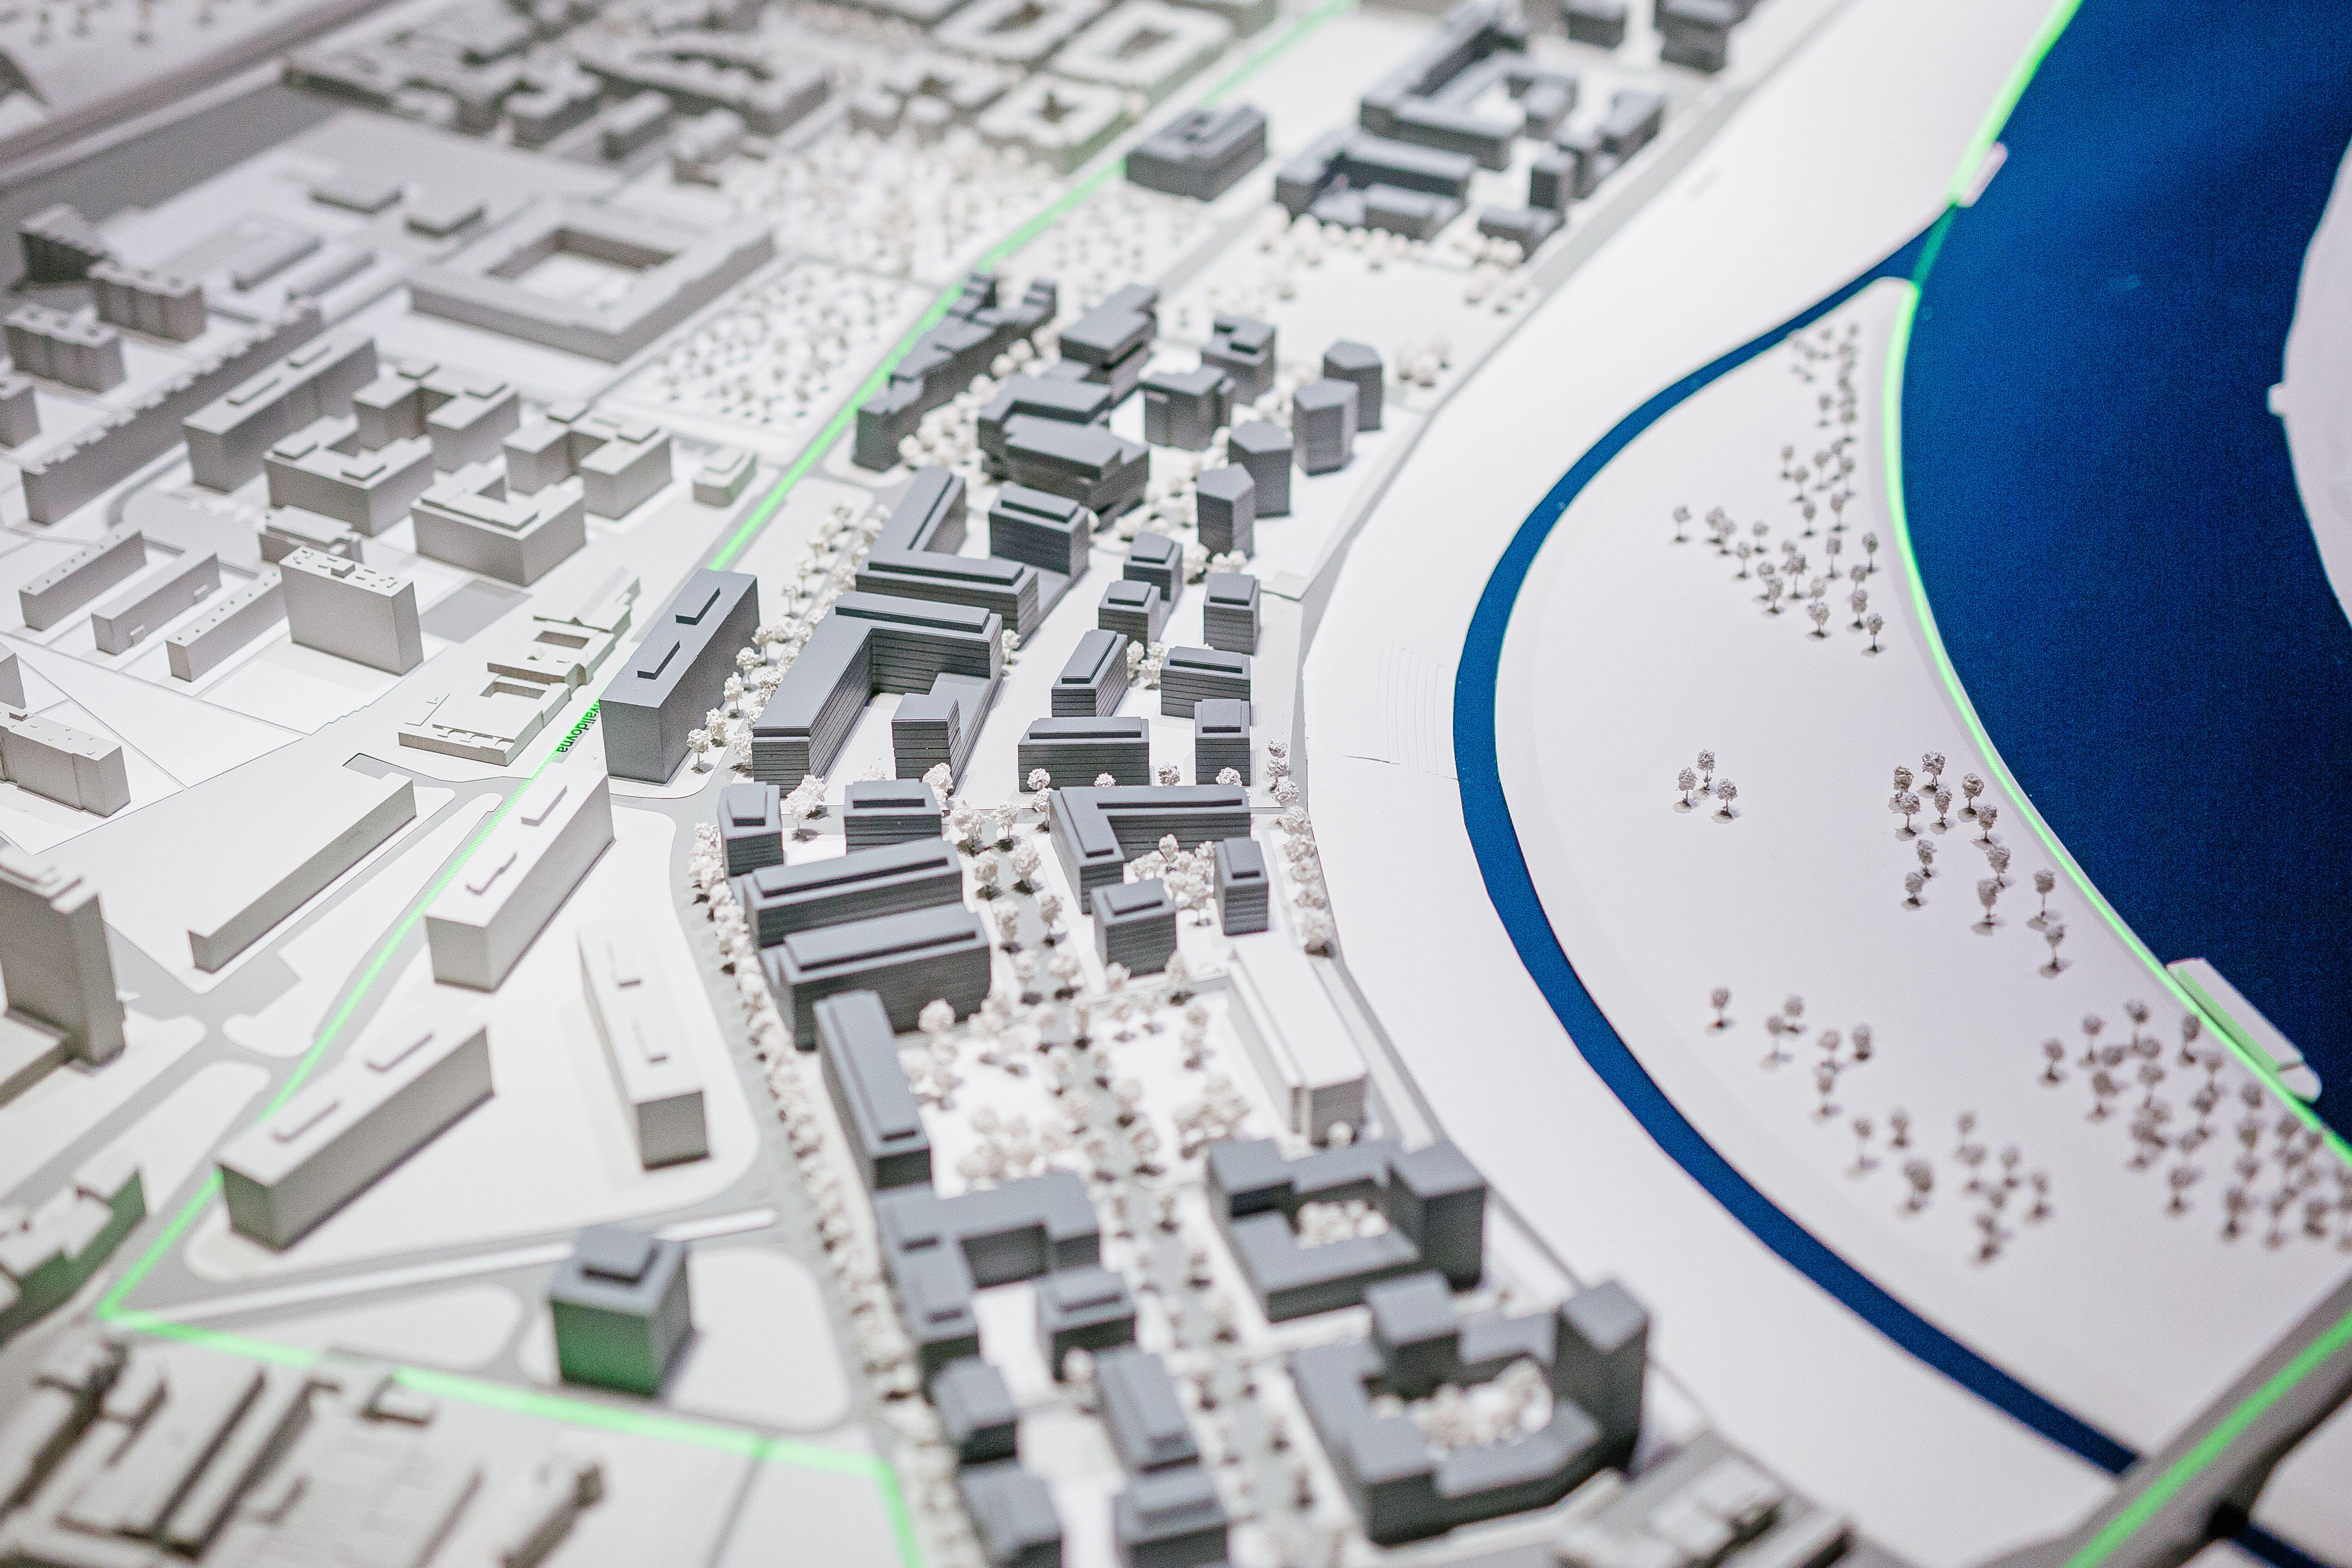
\includegraphics[width=\linewidth]{figures/rohan1.jpg}
        \caption{Highlited area \cite{iprRohanImages}}
        \label{fig:rohanhighlight}
    \end{subfigure}
    \begin{subfigure}[t]{0.49\linewidth}
        \centering
        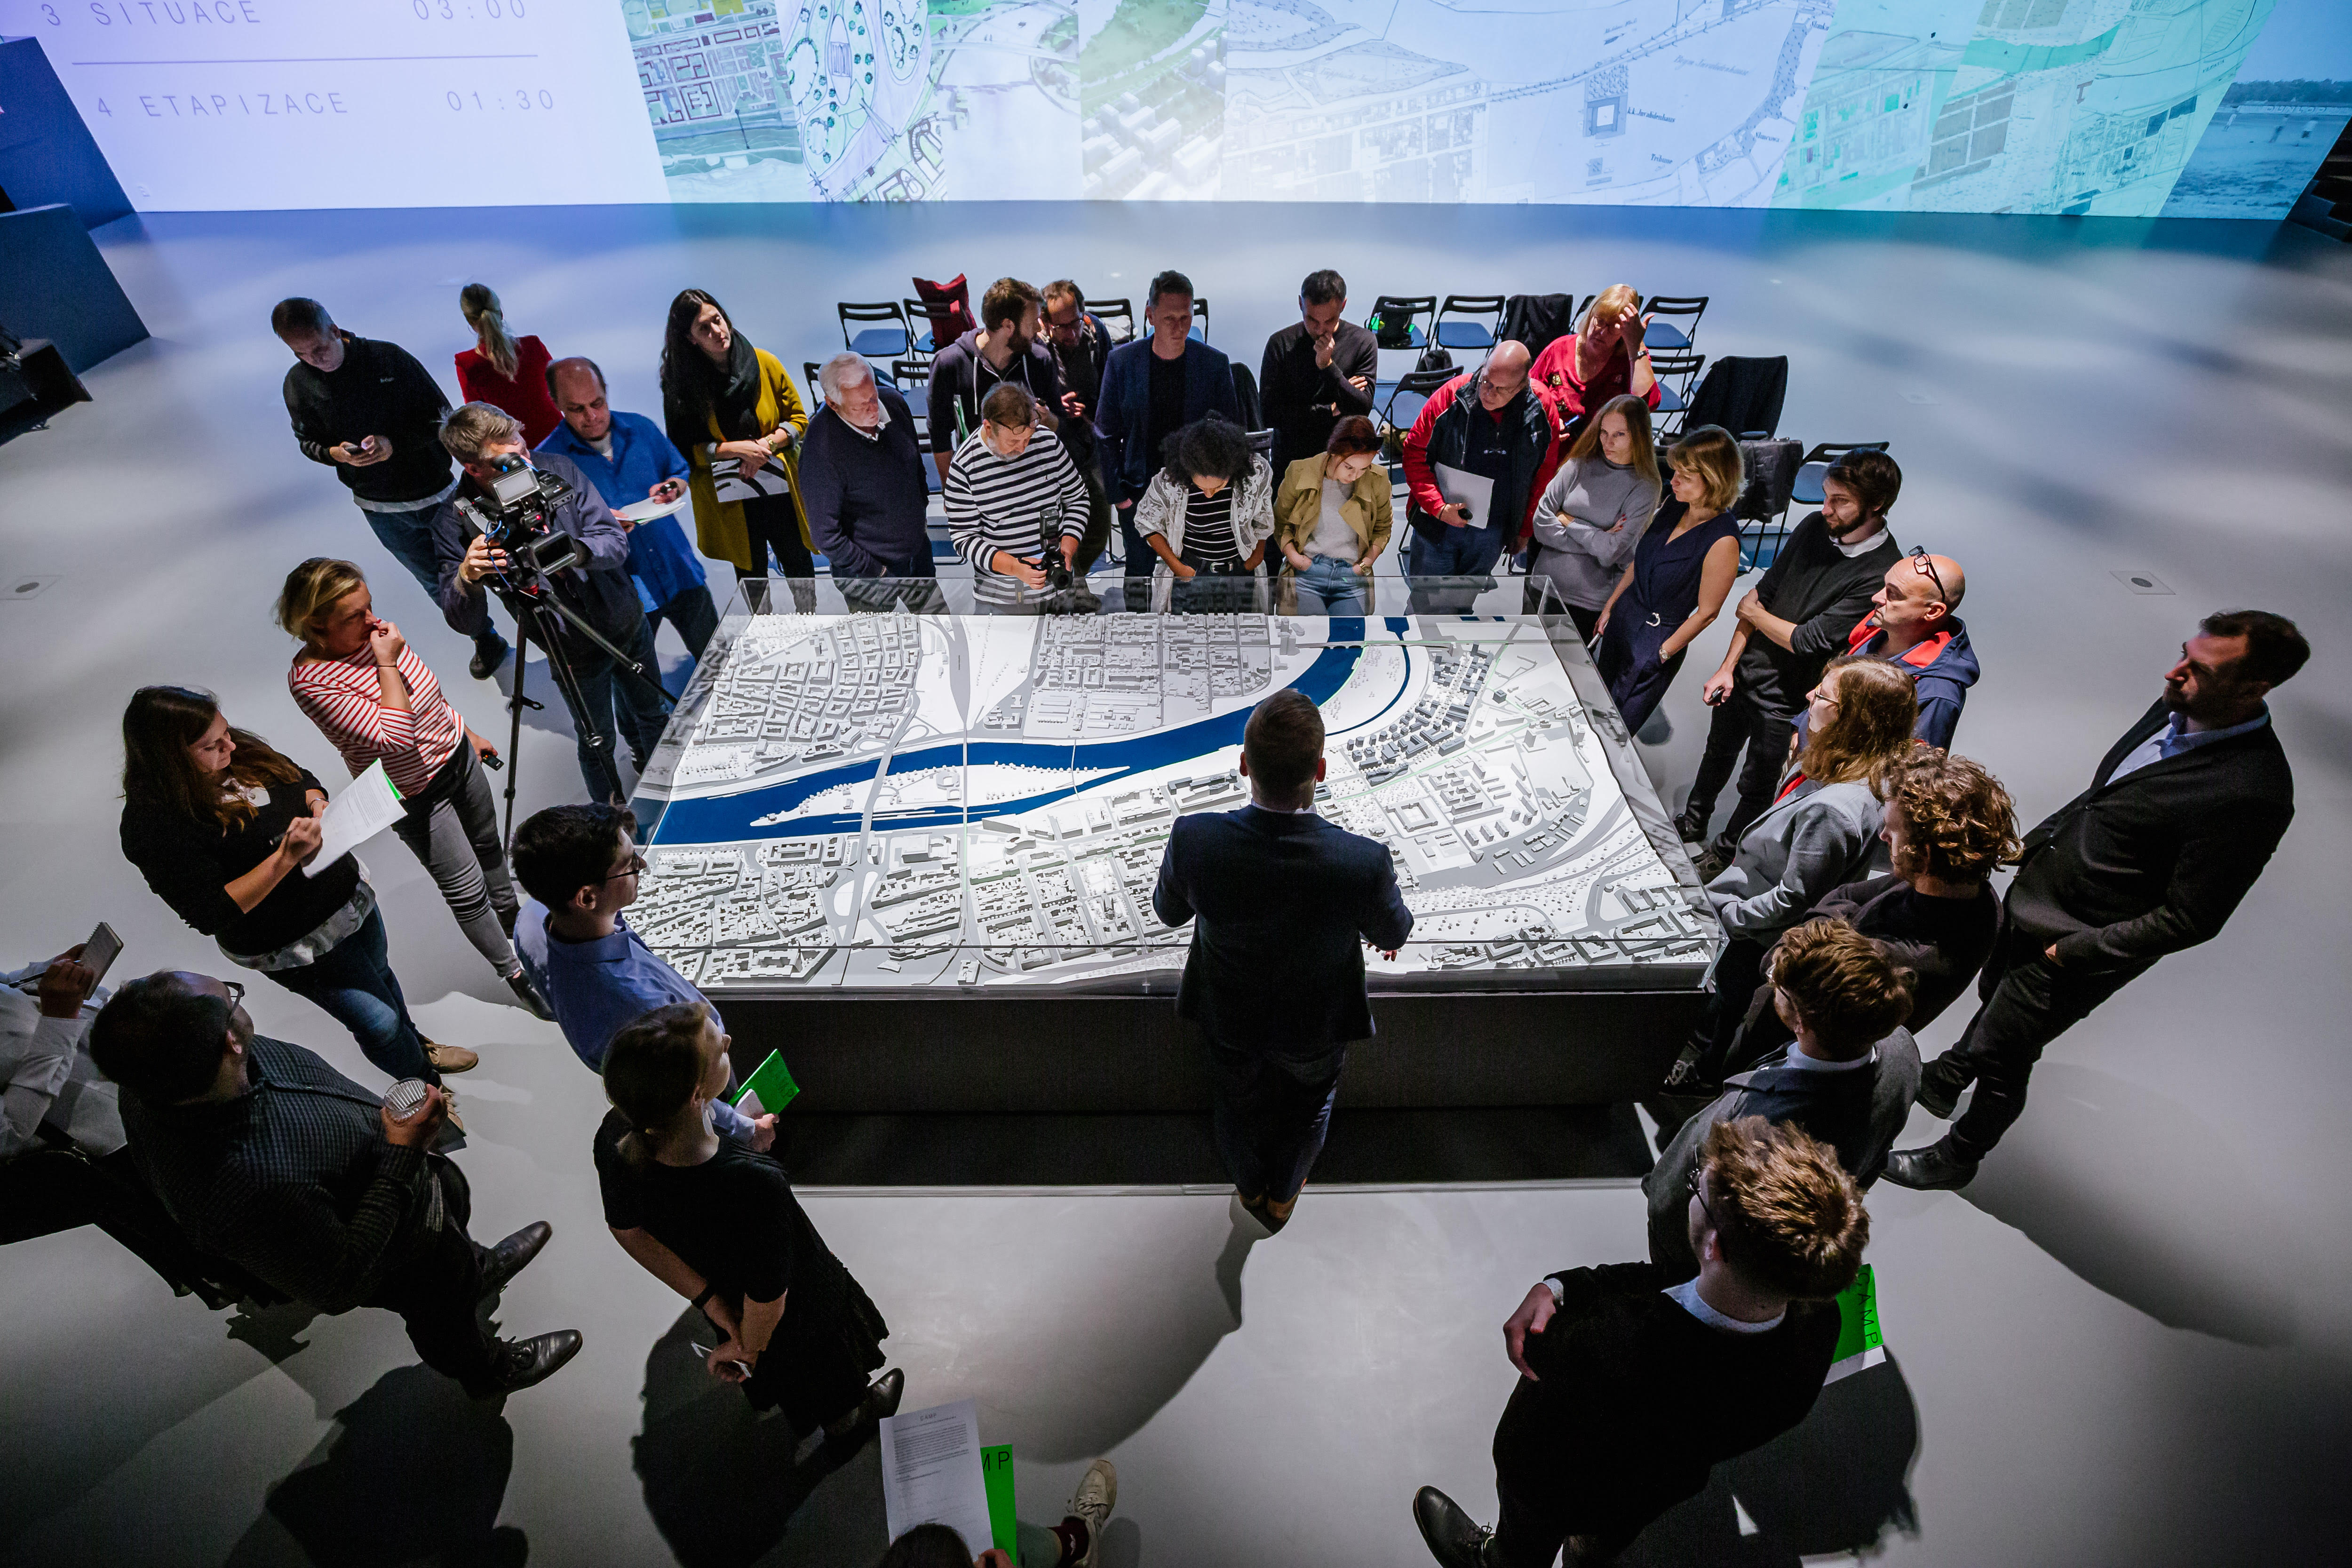
\includegraphics[width=\linewidth]{figures/rohan3.jpg}
        \caption{Physical model \cite{iprRohanImages}}
        \label{fig:rohanmodel}
    \end{subfigure}
    \caption{Rohanský ostrov: nový Karlín? in CAMP}
    \label{fig:rohan}
\end{figure}


\section{Purely Virtual Visualization Tools}
Purely virtual visualization tools are usually a variation of geographic information system (ArcGis, QGIS), but there are a few notable exceptions (kepler.gl, Movement). 

\subsection{Applications}
This section presents the available geospatial visualization applications. As is evidenced by the following list of available applications, the dominant trend in geographic visualization is to move the presentation to the web environment. That has a few advantages:
\begin{itemize}
    \item no need to install any desktop applications
    \item multiplatform apps by default
    \item easily sharable content (it is already on the web)
\end{itemize}

\paragraph{ArcGis} 
Esri offers a range of GIS products under the name of ArcGIS \cite{esriArcgis}. It is a full suite of software for geospatial visualization and analysis. ArcGIS Urban focuses on urban data, visualization, and planning. It is a web-based application. As it is commercial software with full-time support, it is a widely popular solution used by local authorities. ArcGis supports a wide range of proprietary formats (namely ArcIMS, DGN, DWG, DXF, and a range of raster formats). 

\paragraph{QGIS} An open-source alternative to ArcGIS is QGIS \cite{QGISsoftware} --- a tool for creating, viewing, and editing geospatial information. It supports a wide range of formats (Esri Shapefiles, ArcInfo files, MapInfo files, .csv, OpenStreetMap data, PostGis data together with a group of database-based file formats). There is a QGIS plugin, Qgis2threejs, which provides a way to view 3D content in browser, but it appears that the only supported input format is .hgt - DEM (Digital elevation model) format. From version 3.0, there is built-in support for 3D content; supported formats are mostly Esri Shapefiles and raster formats (e.g. GeoTiff). It is possible to export static images as well as short animations created from time-series data. The current capabilities of the program do not allow to customize the styling of the outputs. 

\paragraph{kepler.gl}
Kepler.gl \cite{uberKepler} is an open-source visualization application developed by vis.gl \cite{visgl}. The tool was created and popularized in collaboration with Uber; the main focus is scalability and good performance. The tool is based on Deck.gl, also made by vis.gl, a WebGL-based rendering framework optimized for big data visualizations. The application uses a concept of layers and filters for displaying the imported data. Each layer is an isolated entity with its own base geometry (lines, arcs, points, hex or rectangular grid, heatmap, etc.) and style. 
The application uses OpenStreetMap \cite{openstreetmap} and Mapbox \cite{mapbox} data as a source for 2D maps and 3D models of buildings. The only missing 3D component is the terrain height. It is possible to use Kepler.gl as a Python library for visualization inside Jupyter Notebooks. The supported formats include CSV, GeoJSON, and proprietary JSON-based application format. 

\paragraph{Movement}
This application was also developed by vis.gl in collaboration with Uber \cite{uberMovement}. The primary focus of this application is the visualization of transport-related data. This project stands on the border of visualization and data analysis. Unlike the previous examples, this application was developed to present a fixed set of curated datasets. The goal is to help cities (they operate only in a limited number of cities) to reduce congestion, emissions, and improve road safety.

\paragraph{Cesium}
Cesium \cite{ce2019cesiumjs} is a platform for building geospatial applications. It provides a way to push 3D content to both web (CesiumJS) and Unreal Engine. A part of the services is a platform called Ion, which automatically tiles and optimizes the content for both web and the game engine and offers a library of assets such as images, terrain, and building models. Cesium offers a free plan with a limited amount of data. However, the platform is targeted towards commercial projects and offers pre-paid plans with higher bandwidth.

\subsection{Frameworks}
\label{sec:frameworks}
In terms of visualization frameworks, there are several existing solutions. There is a slight difference between the previous examples and these frameworks --- the frameworks are not standalone visualization solutions. The visualization frameworks usually provide a set of features (data management, rendering, etc.) used throughout the visualization pipeline. 

\paragraph{3DCityDB}
3DCityDB \cite{yao20183dcitydb} is a framework oriented towards effective storing, analysis, and export of the urban data. Part of the toolkit is also a visualization client, but the framework is mainly oriented towards data management. The idea behind this framework is the use of the CityGML standard as the base scheme for the data representation. The framework supports export into several formats, such as Collada, glTF, and KML.

\paragraph{Vis.gl Frameworks}
Vis.gl \cite{visgl} develops several web-based frameworks for visualization. Deck.gl is a WebGL-based rendering framework for visual exploratory data analysis of large geospatial datasets. It's built to be compatible with React (app flow and UI) and Mapbox (source of the base map). A more general-purpose visualization framework is Luma.gl, also a WebGL-based toolkit. To provide a way for plotting various data in 2D, vis.gl developed a library React-vis. As the name already suggests, it is built to be compatible with the React app model.

\paragraph{Blender GIS and Up3date}
Several plugins allow for the import of GIS data into Blender, namely Blender GIS \cite{blendergis} or Up3date \cite{up3date}, which are both still maintained. The supported files include CityJSON, Shapefile vector, raster image, GeoTIFF DEM, OpenStreetMap. 


